\documentclass[journal]{IEEEtran}
\usepackage[a5paper, margin=10mm, onecolumn]{geometry}
\usepackage{lmodern} 
\usepackage{tfrupee} 
\setlength{\headheight}{1cm}
\setlength{\headsep}{0mm}   

\usepackage{gvv-book}
\usepackage{gvv}
\usepackage{cite}
\usepackage{amsmath,amssymb,amsfonts,amsthm}
\usepackage{algorithmic}
\usepackage{graphicx}
\usepackage{textcomp}
\usepackage{xcolor}
\usepackage{txfonts}
\usepackage{listings}
\usepackage{enumitem}
\usepackage{mathtools}
\usepackage{gensymb}
\usepackage{comment}
\usepackage[breaklinks=true]{hyperref}
\usepackage{tkz-euclide} 
\usepackage{listings}                             
\def\inputGnumericTable{}                                 
\usepackage[latin1]{inputenc}                                
\usepackage{color}                                            
\usepackage{array}                                            
\usepackage{longtable}                                       
\usepackage{calc}                                             
\usepackage{multirow}                                         
\usepackage{hhline}                                           
\usepackage{ifthen}                                           
\usepackage{lscape}
\usepackage{xparse}

\bibliographystyle{IEEEtran}

\title{1.5.30}
\author{EE25BTECH11043 - Nishid Khandagre} % Replace with your name

\begin{document}
\maketitle

\renewcommand{\thefigure}{\theenumi}
\renewcommand{\thetable}{\theenumi}

\numberwithin{equation}{enumi}
\numberwithin{figure}{enumi} 

\textbf{Question}:\\
If the coordinates of one end of a diameter of a circle are $\myvec{2\\3}$ and the coordinates of its centre are $\myvec{-2\\5}$, then the coordinates of the other end of the diameter are
\\

\textbf{Solution: }
Let the coordinates of one end of the diameter be $\vec{A} = \myvec{2 \\ 3}$.\\
Let the coordinates of the centre of the circle be $\vec{C} = \myvec{-2 \\ 5}$.\\
Let the coordinates of the other end of the diameter be $\vec{B} = \myvec{x \\ y}$.\\

Since the centre of the circle is the midpoint of the diameter, we can use the midpoint formula.\\

The midpoint formula states that if $\vec{C}$ is the midpoint of $\vec{A}$ and $\vec{B}$, \\


then $\vec{C} = \frac{\vec{A} + \vec{B}}{2}$.


Therefore, we have: 
\begin{align}
2\vec{C} = \vec{A} + \vec{B} \\
\vec{B} = 2\vec{C} - \vec{A}
\end{align}


Now, substitute the given coordinates into the equation:
\begin{align}
\myvec{x \\ y} &= 2 \myvec{-2 \\ 5} - \myvec{2 \\ 3} \\
&= \myvec{2 \times (-2) \\ 2 \times 5} - \myvec{2 \\ 3} \\
&= \myvec{-4 \\ 10} - \myvec{2 \\ 3} \\
&= \myvec{-4 - 2 \\ 10 - 3} \\
&= \myvec{-6 \\ 7}
\end{align}


Thus, the coordinates of the other end of the diameter are $\myvec{-6 \\ 7}$

\begin{figure}[H]
   \centering
  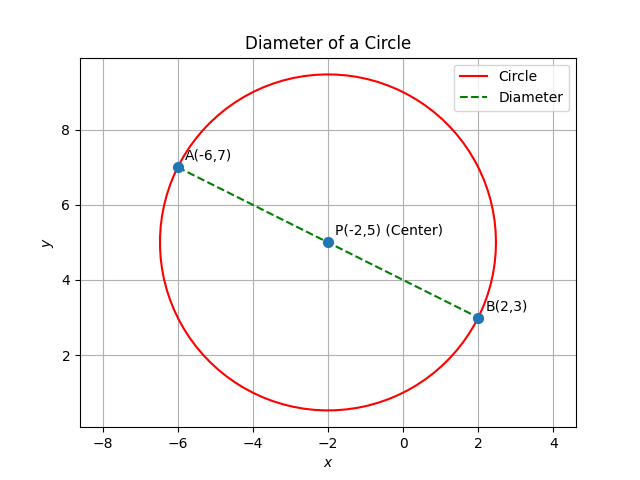
\includegraphics[width=0.7\columnwidth]{figs/fig1.png}
   \caption{}
   \label{fig:1}
\end{figure}

\end{document}